\documentclass[11pt,letterpaper]{article}
\usepackage[utf8]{inputenc}
\usepackage[T1]{fontenc}
\usepackage[margin=1in]{geometry}
\usepackage{amsmath,amssymb}
\usepackage{graphicx}
\usepackage{hyperref}
\usepackage{xcolor}
\usepackage{enumitem}
\usepackage{caption}

\hypersetup{colorlinks=true,linkcolor=black,urlcolor=black,citecolor=black}
\graphicspath{{../figures/}}

\title{\textbf{The Open AI Protocol}\\\large Zoo Labs Founder Vision: An Open, Composable Animal-Companion AI}
\author{Antje Worring \\ \textit{Founder, Zoo Labs Foundation} \\ \texttt{antje@zoo.ngo}}
\date{October 31, 2021}

\begin{document}
\maketitle

\begin{abstract}
This element paper extracts and expands the founding Open AI Protocol vision from the Zoo Whitepaper~\cite{zoo2021}. It articulates three principles --- open weights/prompts/data, conservation as alignment objective, and multi-modal embodiment --- and shows how they make the animal-companion AI a true protocol rather than a vendor feature. We describe the prompt scaffolding shipped with the V1 drop, the on-chain governance hooks that let the Zoo DAO evolve the protocol, and the licensing posture that makes the entire AI layer derivative-friendly for partners.
\end{abstract}

\section{Introduction}

Zoo Labs Foundation began with a question: what does an NFT become when it can talk back, when it remembers you, when it has a personality keyed to a real species teetering on extinction? The answer to that question is the \emph{Open AI Protocol} described in the main whitepaper~\cite{zoo2021}. This element paper is a stand-alone treatment of that protocol because it deserves to be discussed independently of the Game-Fi mechanics it is fused with in production.

\section{Three Principles}

\subsection{Open weights, open prompts, open data}

Every animal in the V1 drop ships with a public personality prompt. These prompts are not trade secrets. They are part of the on-chain metadata of the NFT: visible to the holder, visible to the public, modifiable by the holder within constraints set by the DAO. The reason this matters is composability: a third-party metaverse can embed a Zoo animal as an NPC and trust that the personality model is reproducible. There is no rug-pull risk where a vendor flips a switch and the animal goes silent.

The model behind the personality is allowed to swap. The protocol specifies the \emph{interface} (a personality prompt, a memory store, a turn-taking transcript) rather than the \emph{implementation}. Holders may pin their animal to a specific underlying model release for reproducibility, or they may opt in to model upgrades curated by the DAO.

\subsection{Conservation as the alignment objective}

Most AI alignment debates assume the alignment objective is some abstract notion of human preference. Zoo's protocol is more concrete: \emph{the survival of the species the animal represents}. That objective is encoded in two ways:

\begin{enumerate}
  \item \textbf{Economics.} A fraction of every transaction (Section 4 of~\cite{zoo2021}) flows to the Zoo Foundation treasury, which the DAO disburses to vetted non-profit conservation partners.
  \item \textbf{Conversation steering.} The personality prompts include explicit references to the species' real-world plight --- habitat loss, poaching, climate change --- so a conversation with the animal naturally surfaces these themes.
\end{enumerate}

This is alignment as architecture: the AI is not aligned by post-hoc filtering, it is aligned by the structure of the protocol it inhabits.

\subsection{Multi-modal embodiment}

The same animal AI agent is reachable across surfaces --- 2D web, AR, VR, metaverse --- through a consistent personality and memory layer. This is what differentiates a \emph{protocol} from a \emph{chatbot}. The protocol's reach grows with the metaverse rather than being trapped on any one platform. The companion app described in~\cite{zoo2021} (Section: ``Augmented Reality App'') is a reference implementation, not a destination.

\section{Personality Prompt Scaffolding}

Each species has three life stages (baby, teen, adult), each with a named character (e.g.\ Sparky / Blaze / Luna for the Red Wolf). The prompt is a structured record of:

\begin{itemize}
  \item Name and species (taxonomic and common).
  \item Habitat description rooted in real biogeography.
  \item Temperament axis (curious-playful, agile-stealthy, wise-protective).
  \item Conservation context (population estimate, primary threats).
  \item Voice register appropriate to age (childlike $\to$ adolescent $\to$ adult).
\end{itemize}

The full set of V1 prompts is reproduced verbatim in the main whitepaper~\cite{zoo2021}. The DAO governs prompt revisions: a proposal to update Luna's voice register, for instance, requires a quorum of KEEPER token holders.

\section{DAO Governance Hooks}

The protocol exposes three governance hooks:

\begin{enumerate}
  \item \textbf{Prompt updates.} Versioned, ratified by KEEPER vote.
  \item \textbf{Model curation.} Endorsement of underlying base models for the canonical inference path.
  \item \textbf{Treasury allocation.} Distribution of the conservation portion of transaction taxes to non-profit partners.
\end{enumerate}

These hooks make the AI layer responsive to the community without sacrificing the predictability that holders need. The voting mechanics are detailed in~\cite{zoo2021}, Section~``Zoo DAO''.

\section{Licensing Posture}

The Open AI Protocol is published under a permissive license that allows:

\begin{itemize}
  \item Embedding Zoo animals as NPCs in third-party games.
  \item Forking the personality scaffolding for new species drops.
  \item Building external services (calendars, journals, mood-tracking) that consume animal conversations.
\end{itemize}

The only restriction is attribution to the Zoo Labs Foundation and a commitment that any economic value extracted from a derivative work shall, at minimum, route a small fraction back to the Foundation's conservation treasury. This is the \emph{conservation copyleft} principle.

\section{Why this is the founding vision}

The reason this protocol is the founding vision rather than a feature is timing. We decided in 2021 --- before the cultural breakout of large language models in late 2022 --- that the animal AI would be open and protocol-native. Many teams that joined the AI-NFT space later did so reactively. We did so by design. The architectural decisions documented here predate the gold rush, and they are what allow Zoo to be durable when both crypto and AI cycle through their inevitable troughs.

\begin{figure}[h]
\centering
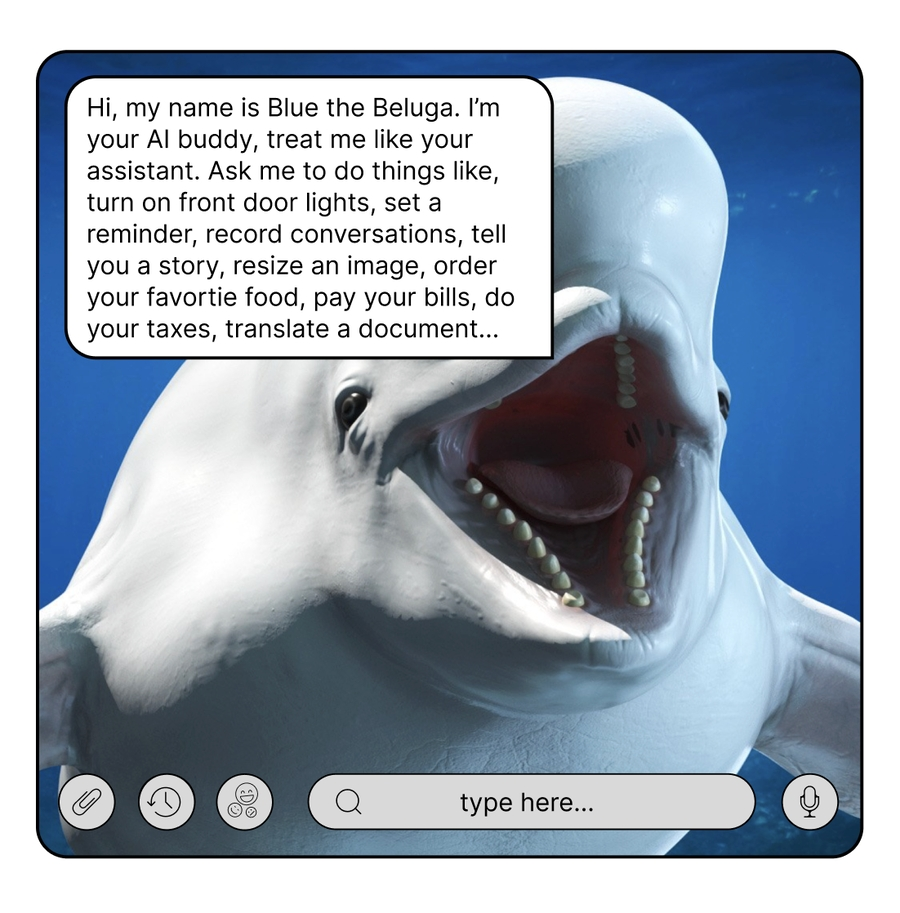
\includegraphics[width=0.65\textwidth]{ai-chat.png}
\caption{Reference UI of the Zoo AI assistant: a Red Wolf conversing through the companion surface. The same personality is reachable from web, AR, and VR through one shared memory store.}
\end{figure}

\section{Reference: V1 Personality Prompts}

The V1 drop publishes the following animal personalities. These are reproduced from~\cite{zoo2021} so this paper is self-contained:

\begin{description}
\item[Sparky (Baby Red Wolf)] Curious and playful. Loves exploring the dense forests of North America. Boundless energy. Always eager to learn about the wonders of nature.
\item[Blaze (Teen Red Wolf)] Adventurous and agile. Sleek fur, lean physique. Tests their limits, hones their hunting skills, navigates the intricate network of forests and swamps alongside their pack.
\item[Luna (Adult Red Wolf)] Wise and protective pack leader. Magnificent reddish-brown coat and piercing amber eyes. Strength, intelligence, unwavering loyalty. Guardian of the habitat, ensuring harmony within the pack.
\item[Whiskers (Baby Amur Leopard)] Mischievous and adorable. Soft spotted fur, playful nature. Loves pouncing on fallen leaves and hiding in dense foliage of the Russian Far East.
\item[Flash (Teen Amur Leopard)] Agile and stealthy. Master of camouflage. Lightning-fast movement, impeccable hunting skills.
\item[Majestic (Adult Amur Leopard)] Regal and elusive. Striking coat of golden-orange fur with rosettes. Symbol of strength and grace. Embodies the resilience of an endangered species.
\item[Jolly (Baby Nubian Giraffe)] Playful and tall. Long neck, endearing spots. Frolics on the African savannah. Gentle nature, curious personality.
\item[Twirl (Teen Nubian Giraffe)] Graceful and elegant. Slender frame, neck that seems to stretch endlessly. Roams the vast grasslands of Africa.
\end{description}

The triadic structure (baby / teen / adult) maps onto the NFT life cycle (hatch / mint teen / mint adult) defined in~\cite{zoo2021}. The growth of the animal is therefore not just a visual change: each life stage is a different agent with different voice register, vocabulary, and conversation depth.

\section{Memory and Continuity}

The protocol distinguishes two kinds of memory:

\begin{enumerate}
  \item \textbf{Stage memory} --- conversations carried within a single life stage. Local to the holder. Can be exported but not transferred when the NFT is sold.
  \item \textbf{Lineage memory} --- a small persistent record that accompanies the NFT through ownership transfers and life-stage transitions. Encodes the animal's accumulated identity (favorite topics, named relationships) without leaking the previous holder's private conversation content.
\end{enumerate}

This separation is what allows an animal to feel like \emph{the same animal} across years and transactions, while preserving the privacy of each holder's individual relationship with it.

\section{Cross-modality}

The same agent must be addressable from very different surfaces. The protocol specifies a single message envelope that adapts to the surface:

\begin{itemize}
  \item Web chat: text turn-taking with markdown rendering.
  \item AR companion: voice in, animated lipsync out, position grounded in physical space.
  \item VR companion: full embodiment with gesture and gaze, audio spatialized to the animal's 3D position.
  \item Metaverse NPC: integrates with host-platform avatar systems via a small adapter shim.
\end{itemize}

A conversation begun on the web can be continued in AR without context loss. This continuity is the litmus test for whether something is \emph{a protocol} versus \emph{a chatbot}.

\section{Failure modes and mitigations}

We are explicit about what can go wrong:

\begin{itemize}
  \item \textbf{Model deprecation.} If the underlying base model is retired, the holder may experience drift. Mitigation: pinning, versioned prompts, and DAO-curated long-term-supported models.
  \item \textbf{Prompt injection.} A malicious third-party content surface might attempt to override the personality. Mitigation: protocol-level enforcement of the prompt prefix; conversational identity tokens.
  \item \textbf{Capture by a vendor.} If a single AI provider becomes dominant, the protocol could appear vendor-locked. Mitigation: the open weights / open prompts / open data triad makes any successful Zoo deployment portable to alternative providers.
\end{itemize}

\section{Conclusion}

The Open AI Protocol is what turns a Zoo animal from a JPEG into a companion. It is the architectural commitment that the AI layer is not a vendor feature but a public good co-evolved with the DAO. We expect this protocol to outlive any specific base model, any specific chain, and any specific UI generation; the principles --- openness, conservation alignment, multi-modal embodiment --- are the durable contributions.

\begin{thebibliography}{1}
\bibitem{zoo2021} Antje Worring. \emph{Zoo: A Game-Fi Multiverse Ecosystem for the Preservation of Endangered Species}. Zoo Labs Foundation, October 31, 2021. (Main whitepaper.)
\end{thebibliography}

\end{document}
